% Encoding: UTF-8
%%%%%%%%%%%%%%%%%%%%%%%%%%%%%%%%%%%%%%%%%%%%%%%%%%%%%%%%%%%%%%%%%%%%%%%%%%%%%%%

%%%%%%%%%%%%%%%%%%%%%%%%%%%%%%%%%%%%%%%%%%%%%%%%%%%%%%%%%%%%%%%%%%%%%%%%%%%%%%%
% $Id: slides.tex 17 2011-02-10 15:21:56Z klugeflo $
%%%%%%%%%%%%%%%%%%%%%%%%%%%%%%%%%%%%%%%%%%%%%%%%%%%%%%%%%%%%%%%%%%%%%%%%%%%%%%%

%%%%%%%%%%%%%%%%%%%%%%%%%%%%%%%%%%%%%%%%%%%%%%%%%%%%%%%%%%%%%%%%%%%%%%%%%%%%%%%
%%
%% Vorlage fuer LaTeX-Beamer
%% gemaess dem Corporate Design der Uni Augsburg
%%
%%%%%%%%%%%%%%%%%%%%%%%%%%%%%%%%%%%%%%%%%%%%%%%%%%%%%%%%%%%%%%%%%%%%%%%%%%%%%%%
%%
%% Changelog:
%%
%% 11/02/10 (FAK) Start
%%
%%%%%%%%%%%%%%%%%%%%%%%%%%%%%%%%%%%%%%%%%%%%%%%%%%%%%%%%%%%%%%%%%%%%%%%%%%%%%%%


%%%%%%%%%%%%%%%%%%%%%%%%%%%%%%%%%%%%%%%%%%%%%%%%%%%%%%%%%%%%%%%%%%%%%%%%%%%%%%%

\documentclass[xcolor=pdftex,dvipsnames,table]{beamer}

%%%%%%%%%%%%%%%%%%%%%%%%%%%%%%%%%%%%%%%%%%%%%%%%%%%%%%%%%%%%%%%%%%%%%%%%%%%%%%%

% Language settings
% IMPORTANT: If you change the language settings, make sure to run
% cleantex prior to any latex/pdflatex to remove all .aux files, else
% latex might fail!
%\usepackage[english]{babel}
%\usepackage[german]{babel}

%\usepackage{graphicx}
\usepackage[utf8]{inputenc}
%\usepackage{mathptmx}

\usepackage{svg}
\usepackage{textcomp}
%\usepackage{german}
\usepackage{tikz}
\usepackage{pgfplots}
\usepackage{booktabs}% http://ctan.org/pkg/booktabs
\newcommand{\tabitem}{~~\llap{\textbullet}~~}
\usetikzlibrary{automata,positioning}
\usetikzlibrary{arrows,automata,shapes,calc}


\graphicspath{{./img/}}
%%%%%%%%%%%%%%%%%%%%%%%%%%%%%%%%%%%%%%%%%%%%%%%%%%%%%%%%%%%%%%%%%%%%%%%%%%%%%%%

\usetheme{fai}

% IMPORTANT/TODO: currently only PDF graphic files should be used, PNG
% or JPEG may harm the Adobe Reader colour palette and result in
% strange display colours.
%\DeclareGraphicsExtensions{.pdf}

%\graphicspath{{./img/}}

%%%%%%%%%%%%%%%%%%%%%%%%%%%%%%%%%%%%%%%%%%%%%%%%%%%%%%%%%%%%%%%%%%%%%%%%%%%%%%%
%% Presentation main settings
%%%%%%%%%%%%%%%%%%%%%%%%%%%%%%%%%%%%%%%%%%%%%%%%%%%%%%%%%%%%%%%%%%%%%%%%%%%%%%%

\title{Handschrifterkennung mit CUDA und C++}
%\subtitle{Optional Subtitle}
\author{Christopher Haug, Dominik Walter}
\institute[Uni Augsburg]{University of Augsburg\\Systems and Networking}
\date[]{\today}


%%%%%%%%%%%%%%%%%%%%%%%%%%%%%%%%%%%%%%%%%%%%%%%%%%%%%%%%%%%%%%%%%%%%%%%%%%%%%%%
%% Main Document starts here
%%%%%%%%%%%%%%%%%%%%%%%%%%%%%%%%%%%%%%%%%%%%%%%%%%%%%%%%%%%%%%%%%%%%%%%%%%%%%%%
\setbeamertemplate{section in toc}[ball]
\setbeamertemplate{subsection in toc}[ball unnumbered]
\setbeamertemplate{subsubsection in toc}[ball unnumbered]
\AtBeginSection []{
	\begin{frame}
		\frametitle{Inhaltsverzeichnis}
		\tableofcontents[currentsection,subsubsectionstyle={show/show/show/shaded}]
	\end{frame}
}

\AtBeginSubsection []{
	\begin{frame}
		\frametitle{Inhaltsverzeichnis}
		\tableofcontents[currentsection,subsectionstyle={show/shaded/shaded}]
	\end{frame}
}

\AtBeginSubsubsection []{
	\begin{frame}
		\frametitle{Inhaltsverzeichnis}
		\tableofcontents[currentsection,subsectionstyle={show/shaded/shaded},subsubsectionstyle={show/shaded/shaded/shaded}]
	\end{frame}
}

\begin{document}
	\frame{\titlepage}
	\begin{frame}
		\frametitle{Aufgabe}
		\begin{columns}
			\begin{column}{0.25\textwidth}
				\includegraphics[width=1\textwidth]{sample.png}
			\end{column}
			\begin{column}{0.05\textwidth}
				\\
				\includegraphics[width=1\textwidth]{arrow.png}\\
				\includegraphics[width=1\textwidth]{arrow.png}\\
				\includegraphics[width=1\textwidth]{arrow.png}\\
				\includegraphics[width=1\textwidth]{arrow.png}\\
				\includegraphics[width=1\textwidth]{arrow.png}\\
				\includegraphics[width=1\textwidth]{arrow.png}
			\end{column}
			\begin{column}{0.4\textwidth}
				\includegraphics[width=1\textwidth]{nn.png}
			\end{column}
			\begin{column}{0.05\textwidth}
				\\
				\includegraphics[width=1\textwidth]{arrow.png}\\
				\includegraphics[width=1\textwidth]{arrow.png}\\
				\includegraphics[width=1\textwidth]{arrow.png}\\
				\includegraphics[width=1\textwidth]{arrow.png}\\
				\includegraphics[width=1\textwidth]{arrow.png}\\
				\includegraphics[width=1\textwidth]{arrow.png}
			\end{column}
			\begin{column}{0.25\textwidth}
				\includegraphics[width=1\textwidth]{prediction.png}
			\end{column}
		\end{columns}
	\LARGE
		\begin{itemize}
			\item Erkennung von handgeschriebenen Zahlen
			\item Neuronales Netz
			\item CUDA und C++
		\end{itemize}
		
	\end{frame}
	
	\begin{frame}
		\frametitle{Training/Testing Dataset}
		\begin{block}{THE MNIST DATABASE of handwritten digits}
		\tabitem 60.000 Trainings-Bilder\\
		\tabitem 10.000 Test-Bilder\\
		\tabitem Auflösung: 28x28\\
		\tabitem IDX-Format\\
		\tabitem Source: http://yann.lecun.com/exdb/mnist/
		\end{block}
		\includegraphics[width=0.15\textwidth]{trainings_sample_example_0.png}
		\includegraphics[width=0.15\textwidth]{trainings_sample_example_1.png}
		\includegraphics[width=0.15\textwidth]{trainings_sample_example_2.png}
		\includegraphics[width=0.15\textwidth]{trainings_sample_example_3.png}
		\includegraphics[width=0.15\textwidth]{trainings_sample_example_4.png}\\
		\includegraphics[width=0.15\textwidth]{trainings_sample_example_5.png}
		\includegraphics[width=0.15\textwidth]{trainings_sample_example_6.png}
		\includegraphics[width=0.15\textwidth]{trainings_sample_example_7.png}
		\includegraphics[width=0.15\textwidth]{trainings_sample_example_8.png}
		\includegraphics[width=0.15\textwidth]{trainings_sample_example_9.png}
		
	\end{frame}


	\begin{frame}
		\frametitle{Feed-Forward / Back-Propagation}
		\includegraphics[width=1\textwidth]{nn.png}
	\end{frame}

	\begin{frame}
		\frametitle{CUDA-Implementierung}
		\begin{columns}
			\begin{column}{0.5\textwidth}
				\underline{Feed-Forward:}
				\begin{itemize}
					\item Eingehende-Kanten ($edges$)
					\begin{itemize}
						\item Thread
						\item Berechnet Kanten-Wert
						\item Speichert in $Shared Memory$
					\end{itemize}
					\item Knoten ($nodes$)
					\begin{itemize}
						\item Thread-Block
						\item Summiert alle Kanten-Werte
						\item Berechnet Knoten-Wert (Sigmoid)
					\end{itemize}
					\item Ausgabe
					\begin{itemize}
						\item Index des höhsten Knoten im $OutputLayer$
					\end{itemize}
				\end{itemize}
			\end{column}
			\begin{column}{0.6\textwidth}
				\includegraphics[width=1\textwidth]{nn.png}
			\end{column}
		\end{columns}
	\end{frame}

	\begin{frame}
		\frametitle{CUDA-Implementierung}
		\begin{columns}
			\begin{column}{0.5\textwidth}
				\underline{Back-Propagation:}
				\begin{itemize}
					\item Ausgehende-Kanten (edges)
					\begin{itemize}
						\item Thread
						\item Berechnet Kanten-Fehler
						\item Speichert in $Shared Memory$
						\item Aktualisiert Kanten-Gewichte
					\end{itemize}
					\item Knoten (nodes)
					\begin{itemize}
						\item Thread-Block
						\item Summiert alle Kanten-Fehler
						\item Berechnet Knoten-Fehler
					\end{itemize}
				\end{itemize}
			\end{column}
			\begin{column}{0.6\textwidth}
				\includegraphics[width=1\textwidth]{nn.png}
			\end{column}
		\end{columns}
	\end{frame}

	\begin{frame}
		\frametitle{C++-Implementierung}
		\begin{columns}
			\begin{column}{0.5\textwidth}
				\begin{itemize}
					\item Aufteilung der Knoten auf n Threads
					\item Jeder Thread berechnet k Knoten-Werte/-Fehler
					\item Bulk-Synchronisation zwischen den Ebenen
				\end{itemize}
			\end{column}
			\begin{column}{0.6\textwidth}
				\includegraphics[width=1\textwidth]{nn.png}
			\end{column}
		\end{columns}
	\end{frame}

	\begin{frame}
		\frametitle{Auswertung CUDA}
		\begin{columns}
			\begin{column}{0.5\textwidth}
				\begin{figure}[htbp]
					\begin{figure}[htbp]
						\begin{minipage}{1\textwidth}
							\begin{tikzpicture}
							\begin{semilogxaxis}[
							width=1.15\textwidth,
							xlabel={Hidden-Nodes},
							ylabel={[s]},
							legend style={at={(0.5,1.05)},anchor=south}
							]
							
							
							\addplot +[mark=] coordinates {
								(1, 0.858043) (2, 0.863491) (4, 0.888018) (8, 0.904576) (16, 0.977727) (32, 1.21229) (64, 1.62353) (128, 2.35729) (256, 3.84786) (512, 7.05504) (1024, 18.0514)
							};
							
							\addplot +[mark=] coordinates {
								(1, 0.622101) (2, 0.618994) (4, 0.609527) (8, 0.624578) (16, 0.617886) (32, 0.608759) (64, 0.617062) (128, 0.681693) (256, 0.636727) (512, 0.761906) (1024, 1.07966)
							};
							
							\legend{Training, Overhead}
							\end{semilogxaxis}
							\end{tikzpicture}
						\end{minipage}
					\end{figure}
				\end{figure}
			\end{column}
			\begin{column}{0.1\textwidth}
			\end{column}
		\begin{column}{0.5\textwidth}
			\begin{figure}[htbp]
				\begin{figure}[htbp]
					\begin{minipage}{1\textwidth}
						\begin{tikzpicture}
						\begin{semilogxaxis}[
						width=1.15\textwidth,
						xlabel={Hidden-Nodes},
						legend style={at={(0.5,1.05)},anchor=south},
						]
						
						
						\addplot +[mark=] coordinates {
							(1, 0.155423) (2, 0.154477) (4, 0.155825) (8, 0.158822) (16, 0.16177) (32, 0.18289) (64, 0.211748) (128, 0.269524) (256, 0.396448) (512, 0.641058) (1024, 1.17412)
						};
						
						\addplot +[mark=] coordinates {
							(1, 0.124953) (2, 0.125682) (4, 0.122199) (8, 0.124556) (16, 0.123301) (32, 0.12453) (64, 0.123628) (128, 0.129924) (256, 0.134051) (512, 0.145165) (1024, 0.171621)
						};
						
						\legend{Testing, Overhead}
						\end{semilogxaxis}
						\end{tikzpicture}
					\end{minipage}
				\end{figure}
			\end{figure}
	\end{column}
		\end{columns}

	\end{frame}

	\begin{frame}
	\frametitle{Auswertung-CUDA / C++}
	\begin{figure}[htbp]
		\begin{figure}[htbp]
			\begin{minipage}{0.6\textwidth}
				\begin{tikzpicture}
				\begin{semilogxaxis}[
				width=1.15\textwidth,
				ylabel={Precision},
				xlabel={Hidden-Nodes},
				legend style={at={(0.5,1.05)},anchor=south}
				]
								
				\addplot +[mark=] coordinates {
					(1, 0.2067) (2, 0.2995) (4, 0.6078) (8, 0.8865) (16, 0.919) (32, 0.9261) (64, 0.9308) (128, 0.9292) (256, 0.9294) (512, 0.9299) (1024, 0.8617)
				};
			
				\end{semilogxaxis}
				\end{tikzpicture}
			\end{minipage}
		\end{figure}
	\end{figure}
	\end{frame}

	\begin{frame}
		\frametitle{Auswertung-CUDA / C++}
		\begin{figure}[htbp]
			\begin{figure}[htbp]
				\begin{minipage}{0.6\textwidth}
					\begin{tikzpicture}
					\begin{axis}[
					width=1.15\textwidth,
					ylabel={Precision},
					xlabel={Learning Rate},
					legend style={at={(0.5,1.05)},anchor=south}
					]
					
					\addplot +[mark=] coordinates {
						(0.02, 0.8905)
						(0.04, 0.905)
						(0.06, 0.9119)
						(0.08, 0.9175)
						(0.10, 0.9209) 
						(0.12, 0.9172)
						(0.14, 0.9218)
						(0.16, 0.9156)
						(0.18, 0.922)
						(0.20, 0.9211)
						(0.22, 0.9202)
						(0.24, 0.9238)
						(0.26, 0.9227)
						(0.28, 0.9169)
						(0.30, 0.92)
					};
					
					\end{axis}
					\end{tikzpicture}
				\end{minipage}
			\end{figure}
		\end{figure}
	\end{frame}


\begin{frame}
	\frametitle{Auswertung-CUDA / C++}
	\begin{columns}
		\begin{column}{0.5\textwidth}
			\begin{figure}[htbp]
				\begin{figure}[htbp]
					\begin{minipage}{1\textwidth}
						\begin{tikzpicture}
						\begin{semilogxaxis}[
						width=1.15\textwidth,
						xlabel={Hidden-Nodes},
						ylabel={[s]},
						legend style={at={(0.5,1.05)},anchor=south,legend
							columns=2},
						]
						
						\addplot +[mark=] coordinates {
							(1, 0.858043) (2, 0.863491) (4, 0.888018) (8, 0.904576) (16, 0.977727) (32, 1.21229) (64, 1.62353) (128, 2.35729) (256, 3.84786) (512, 7.05504) (1024, 18.0514)
						};
						
						\addplot +[mark=] coordinates {
							(1, 0.50572)				
							(2, 0.824613)
							(4, 1.46499)
							(8, 2.74312)
							(16, 5.30326)
							(32, 10.415)
							(64, 20.7259)
							(128, 41.1186)
							(256, 81.9586)
							(512, 166.128)
							(1024, 366.145)
						};
					
						\addplot +[mark=] coordinates {
							(1, 0.496805)
							(2, 0.531907)
							(4, 0.883698)
							(8, 1.54105)
							(16, 3.06804)
							(32, 6.02725)
							(64, 11.047)
							(128, 21.137)
							(256, 42.0224)
							(512, 87.1071)
							(1024, 178.97)
						};
					
						\addplot +[mark=] coordinates {
							(1, 0.495045)
							(2, 0.82754)
							(4, 0.560424)
							(8, 0.951235)
							(16, 1.78632)
							(32, 3.28547)
							(64, 6.36704)
							(128, 12.2491)
							(256, 23.1065)
							(512, 54.1687)
							(1024, 97.8817)
						};
					
						\addplot +[mark=] coordinates {
							(1, 0.649445)				
							(2, 1.28207)
							(4, 2.17531)
							(8, 0.846521)
							(16, 1.42667)
							(32, 2.78434)
							(64, 5.3864)
							(128, 9.64701)
							(256, 18.5158)
							(512, 36.8782)
							(1024, 74.762)
						};
					
						\addplot +[mark=] coordinates {
							(1, 1.41796)
							(2, 2.69709)
							(4, 4.69907)
							(8, 7.97979)
							(16, 2.22552)
							(32, 3.71952)
							(64, 6.3271)
							(128, 13.3198)
							(256, 24.6216)
							(512, 48.7779)
							(1024, 106.235)
						};

						\legend{CUDA, 1-Threads, 2-Threads, 4-Threads, 8-Threads, 16-Threads}
						\end{semilogxaxis}
						\end{tikzpicture}
					\end{minipage}
				\end{figure}
			\end{figure}
		\end{column}
				\begin{column}{0.1\textwidth}
				\end{column}
		\begin{column}{0.5\textwidth}
			\begin{figure}[htbp]
				\begin{figure}[htbp]
					\begin{minipage}{1\textwidth}
						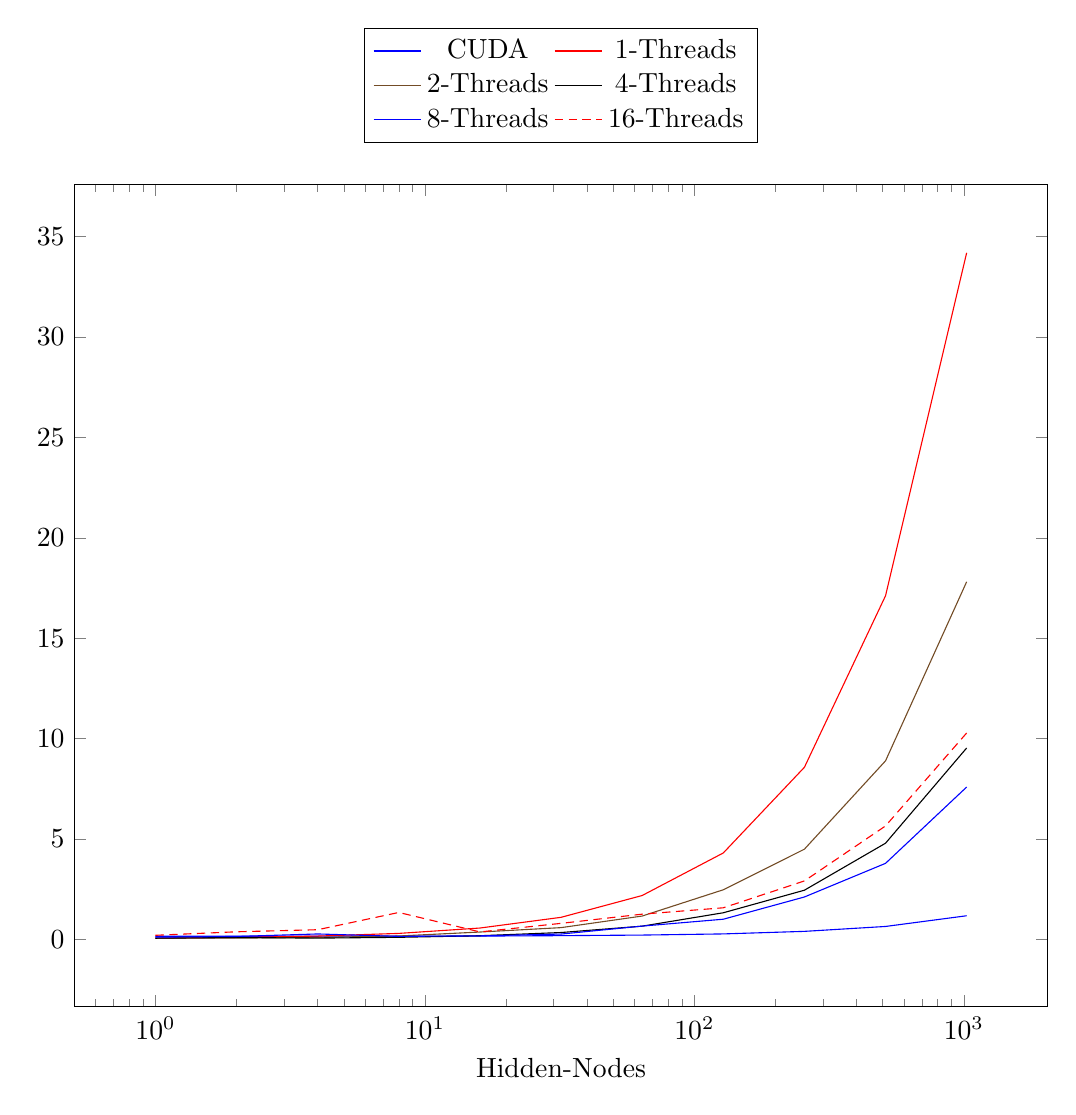
\begin{tikzpicture}
						\begin{semilogxaxis}[
						width=1.15\textwidth,
						xlabel={Hidden-Nodes},
						legend style={at={(0.5,1.05)},anchor=south,legend
							columns=2},
						]
						\addplot +[mark=] coordinates {
							(1, 0.155423) (2, 0.154477) (4, 0.155825) (8, 0.158822) (16, 0.16177) (32, 0.18289) (64, 0.211748) (128, 0.269524) (256, 0.396448) (512, 0.641058) (1024, 1.17412)
						};
						\addplot +[mark=] coordinates {				
							(1, 0.060852)
							(2, 0.094351)
							(4, 0.161698)
							(8, 0.294952)
							(16, 0.562637)
							(32, 1.09585)
							(64, 2.1825)
							(128, 4.30209)
							(256, 8.56935)
							(512, 17.112)
							(1024, 34.1952)	
						};
						\addplot +[mark=] coordinates {
							(1, 0.057688)	
							(2, 0.059385)	
							(4, 0.095331)
							(8, 0.166)
							(16, 0.363225)
							(32, 0.582464)	
							(64, 1.15978)
							(128, 2.46829)
							(256, 4.49106)
							(512, 8.89019)	
							(1024, 17.8091)
						};
						
						\addplot +[mark=] coordinates {
							(1, 0.05551)
							(2, 0.09052)
							(4, 0.060292)
							(8, 0.099768)
							(16, 0.179299)
							(32, 0.338651)
							(64, 0.656342)
							(128, 1.32287)
							(256, 2.44648)	
							(512, 4.78735)
							(1024, 9.52961)
						};			
						\addplot +[mark=] coordinates {
							(1, 0.109625)
							(2, 0.142801)
							(4, 0.267259)
							(8, 0.147465)
							(16, 0.173892)
							(32, 0.262664)
							(64, 0.658467)
							(128, 1.00136)
							(256, 2.10927)
							(512, 3.78485)
							(1024, 7.58448)
						};		
						\addplot +[mark=] coordinates {
							(1, 0.201125)
							(2, 0.375463)
							(4, 0.478362)
							(8, 1.33801)
							(16, 0.368586)
							(32, 0.795383)
							(64, 1.25416)	
							(128, 1.57053)
							(256, 2.90813)
							(512, 5.64799)
							(1024, 10.2777)
						};				
						
	

						
						\legend{CUDA, 1-Threads, 2-Threads, 4-Threads, 8-Threads, 16-Threads}
						\end{semilogxaxis}
						\end{tikzpicture}
					\end{minipage}
				\end{figure}
			\end{figure}
		\end{column}
	\end{columns}
	
\end{frame}

\begin{frame}
	\frametitle{Bottle-Necks}
		C++:
		\begin{itemize}
			\item Synchronisierungsoverhead 
			\item Limitiert durch die Anzahl der CPU-Kerne
			\item Auseinanderlaufende Threads beschränken die Parallelität
		\end{itemize}
	
	
		CUDA:
		\begin{itemize}
			\item Zu viele $Kernel$-Aufrufe
			\item Zu geringer $Workload$
			\item Datenübertragung			
		\end{itemize}
\end{frame}

\end{document}
